\section*{Задание 1}
    Найти решение следующей краевой задачи: 
    \[
        \left\{\begin{split}
            & \frac{1}{r} \frac{\partial}{\partial r} \left( r \frac{\partial u}{\partial r} \right) + \frac{1}{r^2} + \frac{\partial^2 u}{\partial r^2} = 0, \quad 0 < r < 2, \quad 0 < \varphi < 2\pi, \\
            & \frac{\partial u}{\partial r} \big|_{r=2} + 2.5 u|_{r=2} = 2 - \sin \varphi + 3 \sin^2 (2\varphi), \quad 0 < \varphi < 2\pi.
        \end{split} \right.
    \]
    Ищем решение в виде \( u(r, \varphi) = P(r) \cdot \Phi(\varphi) \).
    \[
        \frac{1}{r} \left( r P' \Phi \right)' = - \frac{1}{r^2} P \Phi''
        \quad \Rightarrow \quad
        \frac{r\left(r P'\right)'}{P} = - \frac{\Phi''}{\Phi} = \mu^2
    \]
    \begin{enumerate}
        \item Решим задачу Штурма-Лиувилля для второго равенства.
        \[
            \left\{\begin{split}
                & \Phi'' + \mu^2 \Phi = 0, \\
                & \Phi(\varphi) = \Phi(\varphi + 2\pi).
            \end{split}\right.
            \Rightarrow
            \Phi(\varphi) = C_1 \sin (\mu \varphi) + C_2 \cos (\mu \varphi) 
        \]
        \[
            C_1 \sin (\mu \varphi) + C_2 \cos (\mu \varphi) = C_1 \sin \left(\mu (\varphi+2\pi)\right) + C_2 \cos \left(\mu (\varphi+2\pi)\right)
        \]
        Такое происходит только когда \( \mu_n = n, n \in \mathbb{N}_0 \). \( (n = 0,1,2,\dots) \) Значит решение выглядит так:
        \(
            \Phi_n = A_n \sin (\varphi n) + B_n \cos (\varphi n)
        \).
        \item Найдём решение для первого равенства.
        \[
            r\left( r P' \right)' - \mu_n^2 P = 0.
        \]
        Если \( n = 0 \), то 
        \[
            P_0 = C_1 \ln r + C_2.
        \]
        Задача внутренняя, значит \( \ln r \xrightarrow{r \to 0} -\infty \), значит \( C_1 = 0, P_0 = const \).
        \[
            P_n^{(1)}(r) = r^n, \quad P_n^{(2)}(r) = \frac{1}{r^n}.
        \]
        Т.к. задача внутренняя, то выбираем \( P_n(r) = r^n \).
    \end{enumerate}

    Имеем
    \[
        u(r, \varphi) = \sum_{n=0}^{\infty} u_n(r, \varphi) = B_0 P_0 + \sum_{n=1}^{\infty} r^n \left( A_n \sin (\varphi n) + B_n \cos (\varphi n) \right).
    \]
    Заменим константу \( B_0 P_0 = P_0 \).
    Подставим в граничные условия:
    \[
        \begin{split}
            & \frac{\partial u}{\partial r} \big|_{r=2} + 2.5 u|_{r=2} = \sum_{n=1}^{\infty} n \cdot 2^{n-1} \left( A_n \sin (\varphi n) + B_n \cos (\varphi n) \right) + \\
            & + \frac{5}{2} P_0 + \frac{5}{2} \sum_{n=1}^{\infty} 2^{n} \left( A_n \sin (\varphi n) + B_n \cos (\varphi n) \right).
        \end{split}
    \]
    Распишем то, чему равны граничные условия
    \[
        2 - \sin \varphi + 3 \sin^2 (2\varphi) = 2 - \sin \varphi + 3 \cdot \frac{1 - \cos(2 \cdot 2 \varphi)}{2} = \frac{7}{2} - \sin \varphi - \frac{3}{2} \cos (4\varphi).
    \]
    Сопоставим коэффициенты и найдём их.
    \begin{enumerate}
        \item \(
            \frac{5}{2} P_0 = \frac{7}{2} \Rightarrow P_0 = \frac{7}{5}
        \)
        \item \(
            1 \cdot 2^{1-1} A_1 + \frac{5}{2} \cdot 2^1 A_1 = -1
            \Rightarrow
            6 A_1 = -1
            \Rightarrow
            A_1 = -\frac{1}{6}
        \)
        \item \( 
            4 \cdot 2^{4-1} B_4 + \frac{5}{2} \cdot 2^4 B_4 = -\frac{3}{2}
            \Rightarrow
            72 B_4 = -\frac{3}{2}
            \Rightarrow 
            B_4 = -\frac{1}{48}
        \)
        \item Все остальные коэффициенты равны нулю.
    \end{enumerate}

    \textit{Ответ:} \( u(r, \varphi) = \frac{7}{5} - \frac{1}{6} \sin\varphi - \frac{1}{48} \cos(4 \varphi) \).

    \begin{figure}[H]
        \centering
        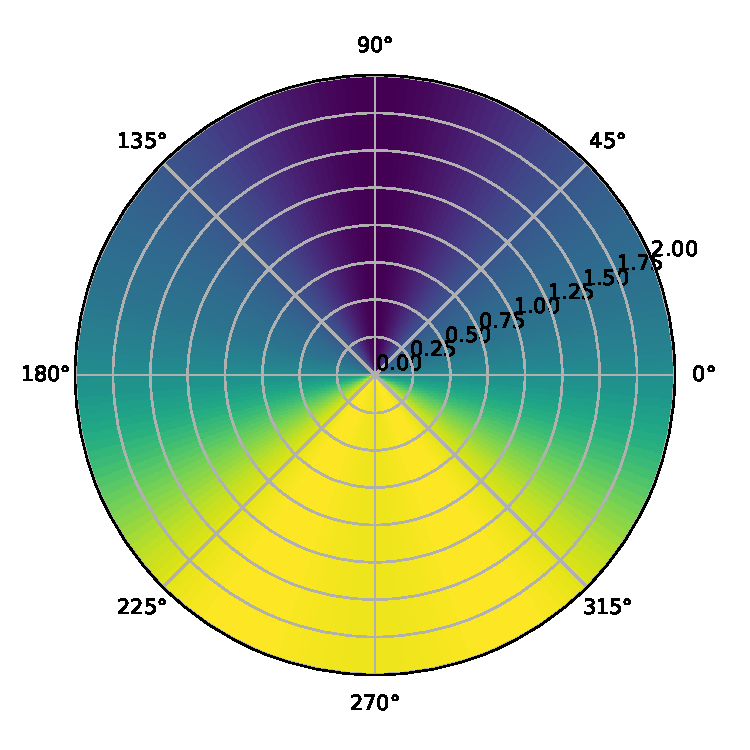
\includegraphics[width=14cm]{p1.pdf}
    \end{figure}

